\input{../../.preambles/01-semester_work}
\input{../../.preambles/10-russian}
\input{../../.preambles/20-math}
\input{../../.preambles/30-physics}
\usepackage{wrapfig}

\newcommand{\rot}{\mathrm{rot}\,}

\begin{document}
\maketitlepage{Факультет электроники и вычислительной техники}{физики}
{Электродинамика}{4}{}{студент группы Ф-369\\Голубев~А.~В.}
{}{доцент Грецов~М.~В.}{}{}

\newpage
\emph{Задача №3.32}: В диэлектрике имеется постоянное магнитное поле 
\( H_0 \). Исследовать монохроматическую волну, которая распространяется:
а) вдоль и б) поперёк магнитного поля. Диэлектрик считать прозрачным и 
немагнитным. 

\emph{Решение:}

\emph{Ответ:}

\newpage

\emph{Задача №3.51}: В однородном, прозрачном и немагнитном диэлектрике 
имеется постоянное магнитное поле \( H_0 \), направленное перпендикулярно 
к его поверхности. На эту поверхность в направлении магнитного поля \( H_0 \) 
падает в вакууме плоская монохроматическая и линейно поляризованная волна, 
интенсивность которой \( J_0 \). Определить интенсивность и состояние 
поляризации отраженной и прошедшей волн.

\emph{Решение:}

\emph{Ответ:}

\newpage

\emph{Задача №3.73}: Показать, что для распространяющейся в волноводе 
\( H \)--волны коэффициент поглощения
\[
	\alpha = \frac{c\kappa^2\theta'}{2k\omega\mu}
	\frac{\oint\limits_{l} 
		\left\{ |H_z|^2 + \frac{k^2}{\kappa^4}|\nabla_2 H_z|^2 \right\}dl
	}{\oint\limits_{S} |H_z|^2 dS}
\]

\emph{Решение:}

Распространяющееся \( H \)--волны в волноводе с поглощением:
\[
	H = H_0 e^{-\alpha}
\]

Используя уравнения Максвелла
\[
	\rot\vec{E} = -\frac{\mu}{c}\pder{\vec{H}}{t};\quad
	\rot\vec{H} = \frac{\eps}{c}\pder{\vec{E}}{t}
\]

положим \( E_z = 0 \) и выразим \( E_x, E_y, H_x, H_y \) через
компоненту \( H_z \):
\[
	\left\{ \begin{array}{ll}
		E_x = i\cfrac{\mu\omega}{c\kappa^2}\cfrac{\partial H_z}{\partial y} \\
		E_y = -i\cfrac{\mu\omega}{c\kappa^2}\cfrac{\partial H_z}{\partial x}
	\end{array} \right. \quad
	\left\{ \begin{array}{ll}
		H_x = \cfrac{ik}{\kappa^2}\cfrac{\partial H_z}{\partial x} \\
		H_y = \cfrac{ik}{\kappa^2}\cfrac{\partial H_z}{\partial y}
	\end{array} \right. \eqno{1}
\]
\[
	\Delta_2 H_z + \kappa^2 H_z = 0 \eqno{2}
\]

где
\(
	\kappa^2 = \cfrac{\omega^2}{v^2} - k^2, 
	v^2 = \cfrac{c^2}{\eps\mu}, 
	\Delta_2 = \cfrac{\partial^2}{\partial x^2} + 
		\cfrac{\partial^2}{\partial y^2} 
\)

Запишем модуль вектора \( \vec{H} \) через его компоненты:
\[
	\vert \vec{H}_t \vert^2 = \vert \vec{H} \vert^2 = 
		H^*_x H_x + H^*_y H_y + H^*_z H_z
\]

с учётом уравнения \( [1] \) получим:
\[
	\vert \vec{H} \vert^2 = \vert H_z \vert^2 + 
		\frac{k^2}{\kappa^2} \vert \nabla_2 H_z \vert^2
\]

Полный поток через сечение волновода можно записать в виде:
\[
	J = \int S^+_z dx dy = \frac{c}{8\pi} \int 
		\left( E_x H^*_y - E_y H^*_x \right) dS
\]

подставляя значения из формулы \( [1] \), получим
\[
	J = \frac{\mu k \omega}{8\pi\kappa^4} \int \vert 
		\nabla_2 H_z \vert^2 dS 
\]

Интегрируя по частям с учётом того, что на контуре сечения 
\( H_z = 0 \)
\[
	J = -\frac{\mu k \omega}{8\pi\kappa^4} \int 
		E^*_z \delta_2 H_z dS
\]

и принимая во внимание уравнение \( [2] \), получим:
\[
	J = \frac{\mu k \omega}{8\pi\kappa^2} \int 
		\vert H_z \vert^2 dS
\]

Энергия поглощаемая стенками волновода не единице его длины за 
единицу времени выражается формулой:
\[
	-\frac{dJ}{dz} = \frac{c\theta'}{8\pi} \oint
		\vert \vec{H}_t \vert^2 dl = \frac{c\theta'}{8\pi} \oint 
		\vert H_z \vert^2 +  \frac{k^2}{\kappa^2} 
		\vert \nabla_2 H_z \vert^2
\]

Деля последнее условие на полный поток найдём коэффициент поглощения:
\[
	2\alpha = \frac{c\kappa^2\theta'}{k\omega\mu}
	\frac{\oint\limits_{l} 
		\left\{ |H_z|^2 + \frac{k^2}{\kappa^4}|\nabla_2 H_z|^2 \right\}dl
	}{\oint\limits_{S} |H_z|^2 dS}
\]


\newpage

\emph{Задача №3.74}: Определить собственные электромагнитные колебания 
в полом (\(\eps = \mu = 1\)) резонаторе, имеющих форму прямоугольного 
параллелепипеда с идеально проводящими стенками, ребра которого равны 
\( a_1, a_2 \) и \( a_3 \). Найти наименьшую собственную частоту.

\emph{Решение:}
\begin{wrapfigure}[10]{l}{0.5\textwidth}
	\vspace{-2ex}
	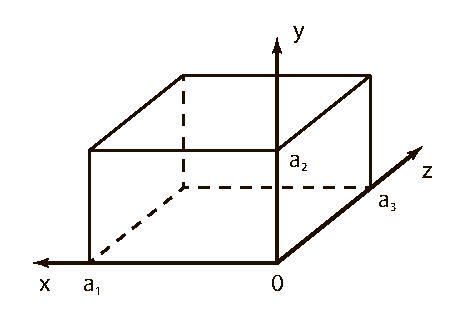
\includegraphics[width=0.5\textwidth]{pdf/image4_4}
\end{wrapfigure}
Воспользуемся волновым уравнение:
\[
	\nabla^2 E + \frac{\omega^2}{c^2} E = 0 \eqno{1}
\]

где \( \nabla^2 = \ppder{}{x} + \ppder{}{y} + \ppder{}{z} \)

Граничные условия: \( E = 0 \) при 
\(
	x = 0, a_1; y = 0, a_2; z = 0, a_3 
\)

Представим решение уравнения \( [1] \) в виде:
\[
	E = A\sin\left( k_x x + \alpha_x \right)
		\sin\left( k_y y + \alpha_y \right)
		\sin\left( k_z z + \alpha_z \right) \eqno{2}
\]

Подставляя его в уравнение \( [1] \), получаем:
\[
	\frac{\omega^2}{c^2} = k^2_x + k^2_y + k^2_z \eqno{3}
\]

Подставляя граничные условия в уравнение \( [2] \), получаем:
\[
	\left\{ \begin{array}{ll}
		\sin\alpha_x = 0 \quad\Rightarrow\quad 
			\alpha_x = 0 \\
		\sin\alpha_y = 0 \quad\Rightarrow\quad 
			\alpha_y = 0 \\
		\sin\alpha_z = 0 \quad\Rightarrow\quad 
			\alpha_z = 0 \\
	\end{array} \right. \quad
	\left\{ \begin{array}{ll}
		\sin k_x a_1 = 0 \quad\Rightarrow\quad 
			k_x = \cfrac{n_1\pi}{a_1} \\
		\sin k_y a_2 = 0 \quad\Rightarrow\quad 
			k_y = \cfrac{n_2\pi}{a_2} \\
		\sin k_z a_3 = 0 \quad\Rightarrow\quad 
			k_z = \cfrac{n_3\pi}{a_3} \\
	\end{array} \right.
\]

Подставляя значения \( k_x, k_y, k_z \) в уравнение \( [3] \) 
найдём собственную частоту:
\[
	\omega^2_{n_1 n_2 n_3} = c^2 \pi^2 \left[ 
		\left( \cfrac{n_1}{a_1} \right)^2 + 
		\left( \cfrac{n_2}{a_2} \right)^2 + 
		\left( \cfrac{n_3}{a_3} \right)^2 \right]
\]

Наименьшая частота будет при условии \( n_1 = n_2 = n_3 = 1 \)
\[
	\omega_{111} = \pm c\pi
		\frac{\sqrt{a^2_1 + a^2_2 + a^2_3}}{a_1 a_2 a_3}
\]

\end{document}